\newpage
\appendix

\section{Anforderungen}

\subsection{Anforderungen aus Kontextebene} \label{anfkontext}
\begin{table}[ht!]
  \begin{tabularx}{\textwidth}{@{}lXp{2cm}@{}}
      \toprule
      ID                & Anforderung & Quelle \\
      \midrule
      % Funktionale Anforderungen
      \textbf{K-FA-1}              &   Das System muss dem Nutzer Zugriff auf den digitalen Zwilling der Anlage gewähren.  & \textit{K-P-1}                \\
      \multicolumn{1}{r}{K-FA-1.1} &  Das Sytem muss dem Nutzer die aktuellen Messewerte in Echtzeit anzeigen.    & \textit{K-P-1.1}\\
      \multicolumn{1}{r}{K-FA-1.2} & Das System muss dem Nutzer die Verortung der Anlage ermöglichen. \\
      \multicolumn{1}{r}{K-FA-1.3} & Das System muss dem Nutzer prädiktive Informationen liefern.\\
      \multicolumn{1}{r}{K-FA-1.4} & Das System muss dem Nutzer die Reaktion auf kritische Zustände in Echtzeit ermöglichen.  & \textit{K-P-1.2}\\
      % Qualitative Anforderungen
      \textbf{K-QA-1}              & Die Architektur des Systems muss dem \ac{sa} die flexible Anpassung an Änderungen erlauben.     & \textit{K-P-2}                \\
      \textbf{K-QA-2}              & Die Architektur des Systems muss dem \ac{sa} die Einbindung neuer Anlagen erlauben.           & \textit{Auftraggeber}                \\
      \textbf{K-QA-3}              &  Die Architektur des System muss dem \ac{sa} die Einbindung von intelligenten Diensten erlauben.  & \textit{K-P-4.1} \\
      \textbf{K-QA-4}              &  Die Architektur des System muss dem \ac{sa} erlauben, das System um Funktionen zu erweitern.  & \textit{K-P-4.1} \\
      % Rahmenbedingungen
      \textbf{K-RA-1}              & Für die Umsetzung des Prototypen muss die SAP Leonardo IoT Foundation verwendet werden.       & \textit{K-P-4} \\
      \textbf{K-RA-2}              & Die Architektur des Systems muss mit \ac{rami} konform sein.      & \textit{K-P-3} \\
      \textbf{K-RA-3}              & Die Simulation muss die Eigenschaften einer Industrie-4.0-Komponente aufweisen.      & \textit{K-P-4.2} \\
      \addlinespace
      \bottomrule
  \end{tabularx}
  \caption{Anforderungen aus Kontextebene}
  \label{kontext_anforderungen}
\end{table}


\subsection{Lösung aus Kontextebene}
\begin{table}[H]
  \begin{tabularx}{\textwidth}{@{}lXp{2cm}@{}}
      \toprule
      ID                & Lösung & Quelle \\
      \midrule
      \textbf{K-L-1}              &   Intelligente Verwaltungsschale für die reale Anlage & \textit{K-P-1}                \\
      \multicolumn{1}{r}{K-L-1.1} &  Der Zustand und zugehörige Daten sollen jederzeit einsehbar sein & \textit{K-P-1.1}\\
      \multicolumn{1}{r}{K-L-1.2} & Der Zustand der Anlage soll bewertbar sein & \textit{K-P-1.2}\\
      \multicolumn{1}{r}{K-L-1.3} & kritische Zustandsveränderungen sollen unverzüglich gemeldet werden & \textit{K-P-1.3}\\
      \textbf{K-L-2}              & IT-Sicht des RAMI 4.0 und Industrie-4.0-Komponente           & \textit{K-P-3}                \\
      \textbf{K-L-3}              &  Prototypische Architekturvorlage für IoT-Projekte & \textit{K-P-3} \\
      \multicolumn{1}{r}{K-L-3.1} &  Messinstrument zur Simulation einer realen Anlage & \textit{K-P-4.2}\\
      \addlinespace
      \bottomrule
  \end{tabularx}
  \label{kontext_losung}
  \caption{Lösungen aus Kontextebene}
\end{table}

% Anforderungen Systemebene
\subsection{Anforderungen aus Systemebene} \label{anf_system}

%\begin{table}[ht!]
  \begin{tabularx}{\textwidth}{@{}lXp{2cm}@{}}
      \toprule
      ID                & Anforderung & Quelle \\
      \midrule
      \endhead
      % Funktionale Anforderungen
      \textbf{S-FA-1} \label{sfa1}             &  Das Messinstrument muss min. alle 5 Sekunden Umgebungsdaten erfassen und verarbeiten können.   &  \textit{Kontext}     \\
      \multicolumn{1}{r}{S-FA-1.1} &   Das Messinstrument muss die Messungen nach der Erfassung kommunizieren können & \textit{\ac{i40}}\\
      \multicolumn{1}{r}{S-FA-1.1} &   Das Messinstrument muss als Entität in einem übergeordneten IT-System vorliegen & \textit{\ac{i40}}\\
      \textbf{S-FA-2}              &   Der Prototyp muss das Messinstrument virtuell als Anlage beschreiben können & \textit{\ac{i40}}        \\
      \multicolumn{1}{r}{S-FA-2.1} &   Der Prototyp muss das Messinstrument eindeutig per \textit{URI} identifizieren können  & \textit{\ac{i40}}\\
      \multicolumn{1}{r}{S-FA-2.2} &   Der Prototyp muss das Messinstrument eindeutig per Koordinaten verorten können  & \textit{\ac{i40}}\\
      \multicolumn{1}{r}{S-FA-2.3} & Der Prototyp muss die Daten (Messwerte und Eigenschaften) der virtuellen Repräsentation halten  & \textit{\ac{i40}} \\
      \multicolumn{1}{r}{S-FA-2.4} & Der Prototyp muss die Grenzüberschreitung der empfangenen Daten erkennen &  \textit{Kontext}\\
      \multicolumn{1}{r}{S-FA-2.5} & Der Prototyp muss die empfangenen Daten kategorisieren &  \textit{Kontext}\\
      \multicolumn{1}{r}{S-FA-2.6} & Der Prototyp muss eine Benachrichtiungs-SMS versenden  &  \textit{Kontext}\\
      \multicolumn{1}{r}{S-FA-2.7} & Der Prototyp muss den Zeitpunkt der letzten gesendeten Nachricht identifizieren (Ausführungsmodus sleep)&  \textit{Kontext} \\
      \multicolumn{1}{r}{S-FA-2.8} & Der Prototyp muss Ereignisse generieren  &  \textit{Kontext}\\
      \multicolumn{1}{r}{S-FA-2.9} & Der Prototyp muss die Anlage an eine Anwendung übergeben &  \textit{Kontext} \\
      \textbf{S-FA-3}              &  Der Prototyp muss dem Nutzer eine Benutzerschnittstelle zur Verfügung stellen    & \textit{Kontext}  \\
      \multicolumn{1}{r}{S-FA-3.1} &  Die Benutzerschnittstelle muss alle Anlagen auf einer Karte verorten \\
      \multicolumn{1}{r}{S-FA-3.2} &  Die Benutzerschnittstelle muss die schnelle Bewertung des Zustands ermöglichen \\
      \multicolumn{1}{r}{S-FA-3.3} &  Die Benutzerschnittstelle muss alle Messwerte auflisten \\
      \multicolumn{1}{r}{S-FA-3.4} &  Die Benutzerschnittstelle muss die Messwerte visualisieren \\
      \textbf{S-QA-1}              & Die Benutzerschnittstelle muss intuitiv sein   \\
      % Qualitative Anforderungen
      \textbf{S-QA-2}              & Die Architektur des Systems muss dem \ac{sa} die horizontale Integration der Anlage ermöglichen.   & \textit{RAMI 4.0} \\
      \textbf{S-QA-3}              &  Die Kommunikation muss nach einem einheitlichen semantischen Modell erfolgen  & \textit{\ac{i40}} \\
      \textbf{S-QA-3}              &  Der Prototyp muss sicher sein  & \textit{\ac{i40}} \\
      \multicolumn{1}{r}{S-QA-3.1}              &  Der Prototyp muss die Verfügbarkeit der Informationen gewährleisten  & \textit{\ac{i40}} \\
      \multicolumn{1}{r}{S-QA-3.2}              &  Der Prototyp muss die Vertraulichkeit der Informationen gewährleisten  & \textit{\ac{i40}} \\
      \multicolumn{1}{r}{S-QA-3.3}              &  Der Prototyp muss die Integrität der Informationen gewährleisten & \textit{\ac{i40}} \\
      \addlinespace
      \bottomrule
      \caption{Anforderungen aus Systemebene}
      \label{system_anforderungen}
  \end{tabularx}

\section{Quelltext und API-Anfragen}

\paragraph{EventPropertySetType}

\begin{lstlisting}
  POST : https://events-sap.cfapps.eu10.hana.ondemand.com/ES/v1/EventPropertySetTypes

  {
  "Name": "cf.devbeta.windmills:windBeaufortSet",
  "PackageName": "cf.devbeta.windmills",
  "DataCategory": "EventData",
  "Properties": [
    {
      "Name": "windBeaufort",
      "Type": "String",
      "PropertyLength": "120",
      "Descriptions": [
        {
          "LanguageCode": "de",
          "Description": "Beaufort Bezeichnungen fuer Windstaerken"
        },
        {
          "LanguageCode": "en",
          "Description": "Beaufort Values for wind strength"
        }
      ]
    }
  ],
  "Descriptions": [
    {
      "LanguageCode": "de",
      "Description": "Set fuer Windstaerken"
    }
  ]
}
\end{lstlisting}

\paragraph{EventTypeBeaufort}

\begin{lstlisting}

  POST: https://events-sap.cfapps.eu10.hana.ondemand.com/ES/v1/EventTypes

  {
	"Name": "cf.devbeta.windmills:windBeaufortEvent",
	"EventTypeState": "Mutable",
	"Descriptions": [{
		"LanguageCode": "de",
		"Description": "Event type for Beaufort Scale"
	}, {
		"LanguageCode": "de",
		"Description": "Event Typ fuer Beaufort Skala"
	}],
	"PackageName": "cf.devbeta.windmills",
	"PropertySetId": "windBeaufortSet",
	"PropertySetType": "cf.devbeta.windmills:windBeaufortSet",
	"PropertySetDescriptions": [{
		"LanguageCode": "en",
		"Description": "Beaufort Property Set Type"
	}],
	"Statuses": [{
		"EventStatus": "Windstille",
		"Descriptions": [{
			"LanguageCode": "de",
			"Description": "Windstille 1,85 kmh"
		}]
	}, {
		"EventStatus": "leiser_Zug",
		"Descriptions": [{
			"LanguageCode": "de",
			"Description": "- 7,41 km/h"
		}]
	}, {
		"EventStatus": "leichte_Brise",
		"Descriptions": [{
			"LanguageCode": "de",
			"Description": "- 12.96 km/h"
		}]
	}, {
		"EventStatus": "schwache_Brise",
		"Descriptions": [{
			"LanguageCode": "de",
			"Description": "- 20,37 km/h"
		}]
	}, {
		"EventStatus": "maessige_Brise",
		"Descriptions": [{
			"LanguageCode": "de",
			"Description": "- 29.63 km/h"
		}]
	}, {
		"EventStatus": "frische_Brise",
		"Descriptions": [{
			"LanguageCode": "de",
			"Description": "- 40.74 km/h"
		}]
	}, {
		"EventStatus": "starker_Wind",
		"Descriptions": [{
			"LanguageCode": "de",
			"Description": "- 51.86 km/h"
		}]
	},{
		"EventStatus": "steifer_Wind",
		"Descriptions": [{
			"LanguageCode": "de",
			"Description": "- 62.97 km/h"
		}]
	},
	{
		"EventStatus": "Sturm",
		"Descriptions": [{
			"LanguageCode": "de",
			"Description": "- 88.90 km/h"
		}]
	},{
		"EventStatus": "schwerer_Sturm",
		"Descriptions": [{
			"LanguageCode": "de",
			"Description": "- 103.71 km/h"
		}]
	},{
		"EventStatus": "Orkan",
		"Descriptions": [{
			"LanguageCode": "de",
			"Description": "- 118.53 km/h"
		}]
	}],
	"Severities": [{
		"EventSeverity": 1,
		"Descriptions": [{
			"LanguageCode": "en",
			"Description": "High"
		}]
	}, {
		"EventSeverity": 2,
		"Descriptions": [{
			"LanguageCode": "en",
			"Description": "Medium"
		}]
	}, {
		"EventSeverity": 3,
		"Descriptions": [{
			"LanguageCode": "en",
			"Description": "Low"
		}]
	}],
	"Codes": [{
		"EventCode": "EQ12",
		"Descriptions": [{
			"LanguageCode": "en",
			"Description": "Event Code 12"
		}]
	}]
}
\end{lstlisting}

  \section{Anhang 1}

  \begin{table}[h]
    \begin{tabular}{lll}
      \toprule
      Kategorie & Eigenschaft\\
      \midrule
      \multirow[t]{2}{*}{Languages/Buildpacks (SAP supported)} & Node.js  \\
       & Java \\
       \multirow[t]{5}{*}{Languages/Buildpacks (Community supported)} & Python \\
       & PHP \\
       & Ruby \\
       & .NET Core \\
       & viele weitere \\
       \multirow[t]{6}{*}{Storage/Messaging Services} & SAP HANA, inkl. XSA Applications \\
       & MongoDB \\
       & PostgreSQL \\
       & Redis \\
       & RabbitMQ \\
       & Object Store, Unstructured Storage \\
       \multirow[t]{3}{*}{Integrated SSO Secrurity Cloud Connector} & Services für Authentifizierung,\\
       & Single Sign-on \\
       & und On-Premise Integrtion \\
       \multirow[t]{3}{*}{Integrated SSO Secrurity Cloud Connector} & AWS - EU, US East\\
       & Azure - US West  \\
      \bottomrule
      \end{tabular}
      \label{cf_table}
    \caption[Eigenschaften der Cloud-Foundry-Umgebung]{Eigenschaften der Cloud-Foundry-Umgebung \citep[S. 195]{Utecht2018}}
  \end{table}


  \newpage

%\end{table}


\begin{figure}[h]
  \centering
  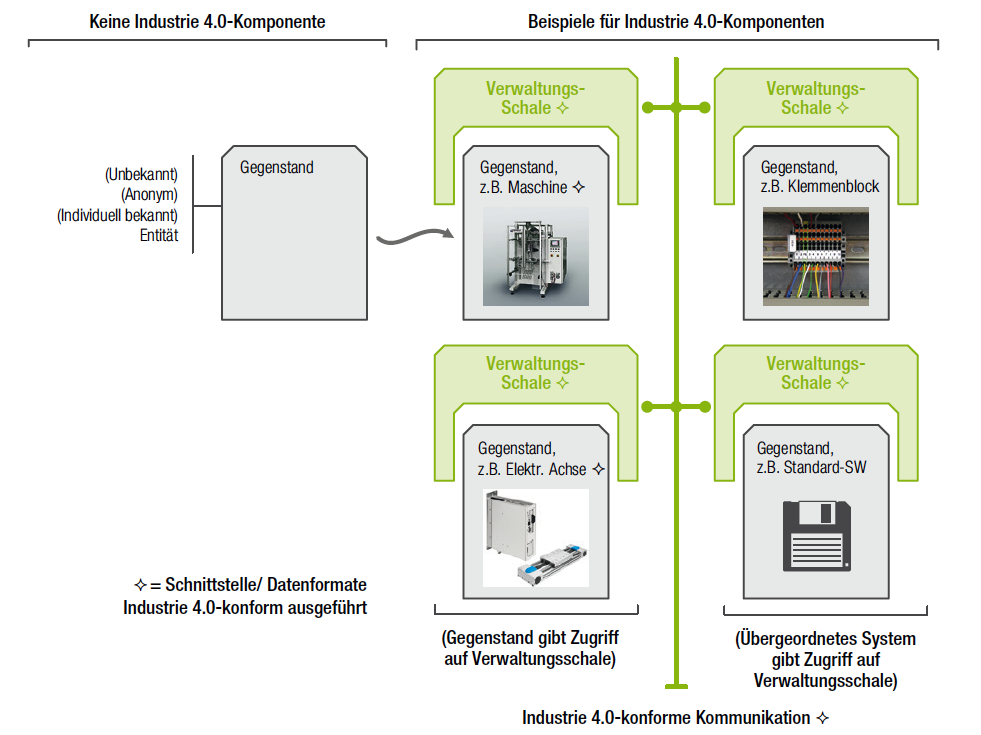
\includegraphics[width=1.1\linewidth]{Bsp_I40_Kompo.png}
  \caption[Beispiele für Industrie-4.0-Komponenten]{Beispiele für Industrie-4.0-Komponenten \citep[S. 54]{BITKOM2015}}
  \label{i40kompo}
\end{figure}

\begin{figure}[h]
  \centering
  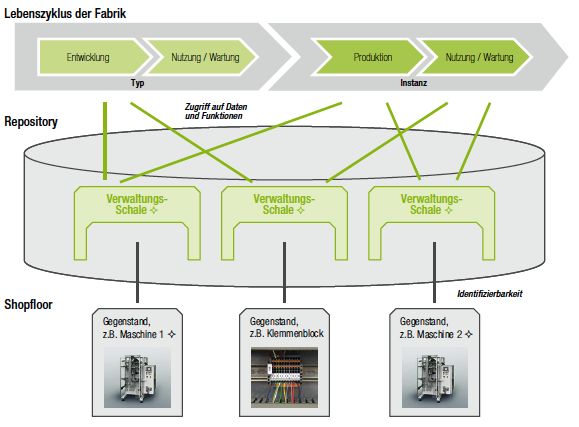
\includegraphics[width=1.1\linewidth]{I40_Lebenszyklus.png}
  \caption[Industrie-4.0-Komponenten im Lebensyklus der Fabrik]{Industrie-4.0-Komponenten im Lebensyklus der Fabrik \citep[S. 56]{BITKOM2015}}
  \label{lifecycle}
\end{figure}

\begin{figure}[h]
  \centering
  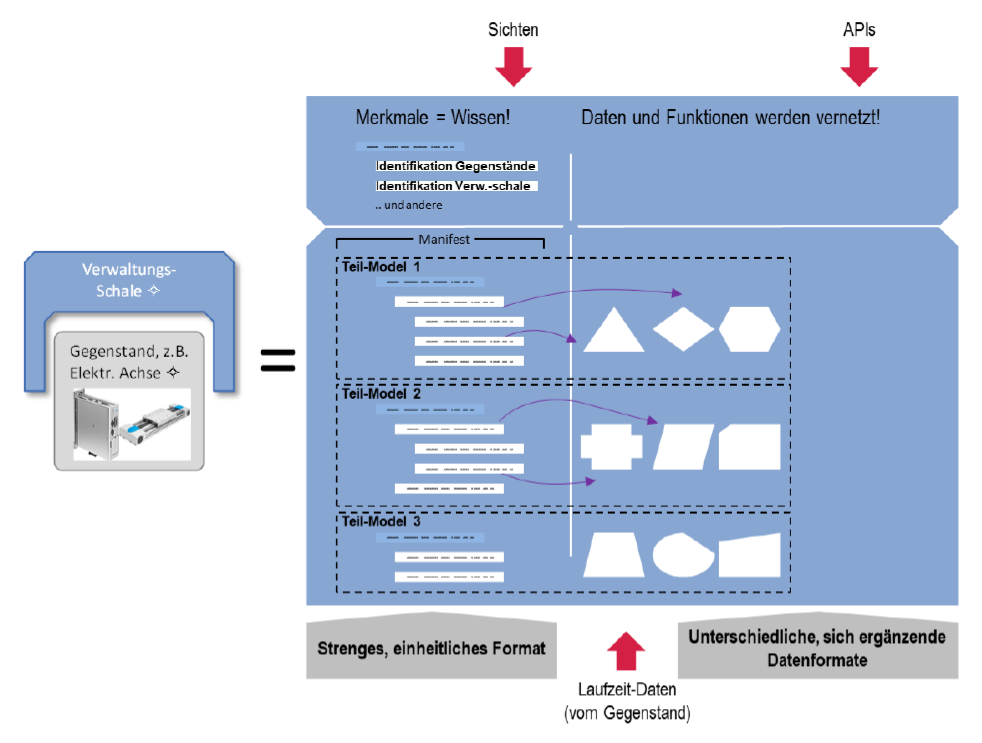
\includegraphics[width=1.1\linewidth]{Struktur_Verwaltungsschale.png}
  \caption[Struktur der Verwaltungsschale]{Struktur der Verwaltungsschale}
  \label{verwaltungsschale}
\end{figure}

\newpage


